\section{Izvedba praktičnog rada}

\subsection{Postavljanje aplikacije}
Za postavljanje aplikacije korišten je predložak \textbf{N-Tier} arhitekture s GitHub platforme dostupan na poveznici \cite{nTierGitHub}.
N-Tier arhitektura višeslojna je klijent-server arhitektura čija je glavna značajka odvajanje aplikacije u fizičke razine i logičke slojeve. U korištenom predlošku, koristi se jedna fizička razina i pet logičkih slojeva kojima je dodan još jedan logički sloj naziva \texttt{PrimeCareMed.Frontend} kao ASP.NET Core Web App projekt u kojem je korišten Razor Pages okvir za izradu aplikacija. Pojedini sloj može koristiti usluge nižeg sloja što je omogućeno dodavanjem ovisnosti na svaki sloj\cite{nTierMicrosoft} \cite{nTierBaeldung}.
Na slici~\ref{fig:nTier} prikazane su ovisnosti projekata u korištenoj arhitekturi. Naprimjer, sloj \texttt{PrimeCareMed.API} može koristiti usluge sloja \texttt{PrimeCareMed.Application} prikazano na slici~\ref{fig:projectDependency}. \\
\begin{figure}[H]
	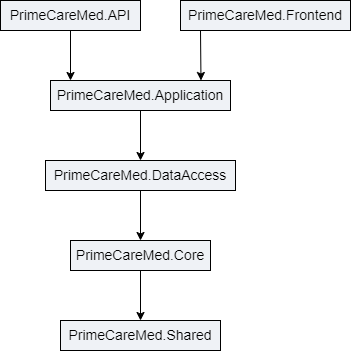
\includegraphics[width=0.6\linewidth,clip=]{assets/Ntier.png}
	\centering
	\caption{Ovisnosti slojeva}
	\label{fig:nTier}
\end{figure}

\begin{figure}[H]
	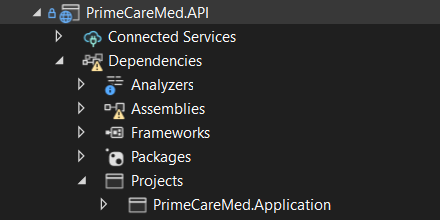
\includegraphics[width=0.6\linewidth,clip=]{assets/projectDependency.png}
	\centering
	\caption{Ovisnosti projekta}
	\label{fig:projectDependency}
\end{figure}

\subsection{Struktura \textit{PrimeCareMed} aplikacije}
Na slici~\ref{fig:primecaremedSolution} prikazana je struktura aplikacije.
\begin{figure}[H]
	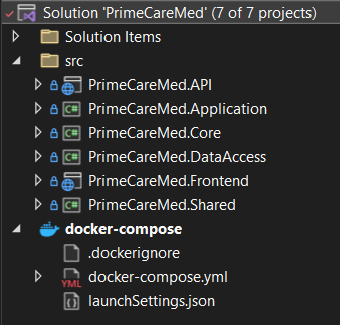
\includegraphics[width=0.6\linewidth,clip=]{assets/StrukturaPrimeCareMed.png}
	\centering
	\caption{Struktura \textit{PrimeCareMed} aplikacije}
	\label{fig:primecaremedSolution}
\end{figure}

Struktura \texttt{src} direktorija sastoji se od šest projekata: \\
\begin{itemize}
\item \texttt{PrimeCareMed.API} - korišten je primarno za pokretanje ostalih nižih slojeva tj. projekata. Također, sadrži direktorij \texttt{Seed} u kojem se nalaze \textit{JSON} (\textit{JSON - JavaScript Object Notation}) datoteke s podatcima korištenima za stvaranje elemenata entiteta.

\item \texttt{PrimeCareMed.Application} - sadrži direktorij \texttt{Models} koji sadrži modele za stvaranje, ažuriranje i prikaz pojedinog entiteta te direktorij \texttt{Service}

\item \texttt{PrimeCareMed.Core} - sadrži klase entiteta i \textit{enumerated} tipove podataka 

\item \texttt{PrimeCareMed.DataAccess} - korišten je za komunikaciju s bazom podataka. Sadrži \texttt{DatabaseContext} klasu u kojoj su definirani entiteti i veze među entitetima te stvorenu migraciju. Također, sadrži direktorij \texttt{Repositories} u kojem se nalaze repozitoriji koji manipuliraju podatcima u bazi podataka.

\item \texttt{PrimeCareMed.Frontend} - sadrži \texttt{wwwroot} direktorij unutar kojeg se nalaze CSS (\textit{CSS - Cascading Style Sheets}) i JavaScript datoteke te poddirektorij \texttt{images} za skladištenje slika korištenih na korisničkom sučelju. Sadrži i poddirektorije za pojedine entitete u kojima se nalaze Razor stranice sa pripadajućim \textit{code-behind} datotekama za usmjeravanje.

\item \texttt{PrimeCareMed.Shared} - sadrži zajedničke datoteke ostalih slojeva
\end{itemize}

\subsection{Baza podataka}
\subsubsection{Struktura relacijske baze podataka}
Na slici~\ref{fig:erDiagram} prikazan je ER (engl. \textit{Entity Relationship}) dijagram relacijske baze podataka u pgAdmin sučelju. Sa slike su izostavljene tablice dobivene korištenjem \texttt{IdentityUser} klase prikazane na slici~\ref{fig:IdentityDatabase}.
\begin{figure}[H]
	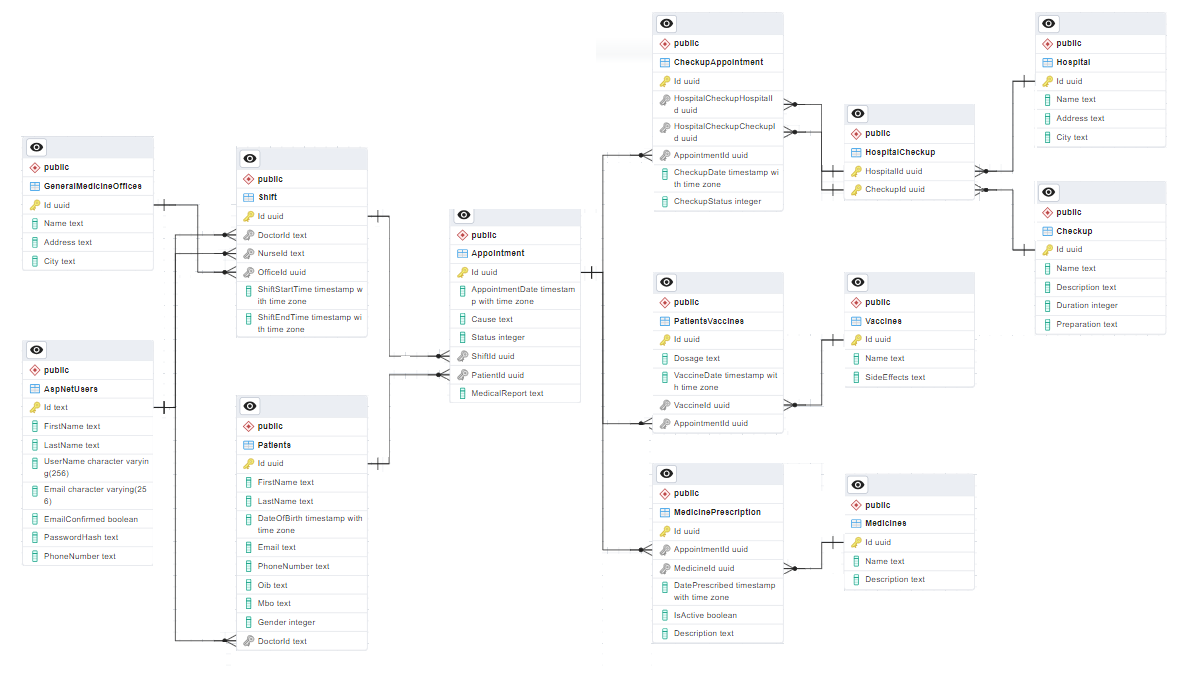
\includegraphics[width=1\linewidth,clip=]{assets/ERdiagram.png}
	\centering
	\caption{Dijagram relacijske baze podataka}
	\label{fig:erDiagram}
\end{figure}

\subsubsection{Entiteti}

Entiteti su definirani u \texttt{PrimeCareMed.Core} projektu.
Na ispisu~\ref{appointmentEntity} prikazana je klasa entiteta \texttt{Appointment}. koja u sebi, uz druge podatkovne članove, sadrži referencu \texttt{Patient Patient} koja predstavlja objekt entiteta \texttt{Patient}, a EntityFrameworkCore stvara \textit{shadow key property} \texttt{PatientId} onog tipa kojeg je primarni ključ u klasi \texttt{Patient}. 
\begin{lstlisting}[caption={Entitet Appointment}, label=appointmentEntity]
using PrimeCareMed.Core.Common;
using PrimeCareMed.Core.Enums;

namespace PrimeCareMed.Core.Entities
{
    public class Appointment : BaseEntity
    {
        public DateTime AppointmentDate { get; set; }
        public string Cause { get; set; }
        public AppointmentStatus Status { get; set; }
        public Shift Shift { get; set; }
        public Patient Patient { get; set; }
#nullable enable
        public string? MedicalReport { get; set; }
        public ICollection<PatientsVaccine>? PatientsVaccines { get; set; } = new List<PatientsVaccine>();
        public ICollection<MedicinePrescription>? MedicinePrescriptions { get; set; } = new List<MedicinePrescription>();
        public ICollection<CheckupAppointment>? CheckupAppointments { get; set; } = new List<CheckupAppointment>();
#nullable disable
    }
}
\end{lstlisting}
Relacija jedan-na-više\cite{oneToMany} omogućena je navedenom referencom i definiranom kolekcijom tipa \texttt{Appointment} u klasi \texttt{Patient} prikazanom na ispisu ~\ref{appointmentCollection}
\begin{lstlisting}[caption={Kolekcija Appointment objekata u klasi Patient}, label=appointmentCollection]
public ICollection<Appointment>? Appointments { get; set; } = new List<Appointment>();
\end{lstlisting}

\subsubsection{Interakcija s bazom podataka}
Interakcija aplikacije s bazom podataka započinje od \texttt{DbContext} klase koja je korištena za dohvaćanje podataka pomoću upita te spremanje novih i ažuriranje postojećih elemenata entiteta. Nakon definiranih entiteta, u \texttt{DatabaseContext.cs} datoteci definirane su kolekcije svih entiteta koje su kasnije korištene za pristup podatcima u bazi podataka. EntityFrameworkCore pomoću \texttt{ModelBuilder} klase automatski stvara jednostavne veze između entiteta. U \texttt{OnModelCreating} metodi korištena je \texttt{ModelBuilder} klasa odgovorna za stvaranje samih modela. Koristi definirane \texttt{DbSet} kolekcije entiteta za stvaranje entiteta i veza iz poznatih podataka. Dodatne konfiguracije mogu biti posebno zapisane u metodi.

\begin{lstlisting}[caption={DatabaseContext.cs datoteka}, label=dbContext]
public DbSet<Medicine> Medicines { get; set; }
public DbSet<GeneralMedicineOffice> GeneralMedicineOffices { get; set; }
public DbSet<Vaccine> Vaccines { get; set; }
public DbSet<Patient> Patients { get; set; }
public DbSet<Shift> Shift { get; set; }
public DbSet<PatientsVaccine> PatientsVaccines { get; set; }
public DbSet<MedicinePrescription> MedicinePrescription { get; set; }
public DbSet<Appointment> Appointment { get; set; }
public DbSet<Hospital> Hospital { get; set; }
public DbSet<Checkup> Checkup { get; set; }
public DbSet<HospitalCheckup> HospitalCheckup { get; set; }
public DbSet<CheckupAppointment> CheckupAppointment { get; set; }

protected override void OnModelCreating(ModelBuilder builder)
{
	builder.ApplyConfigurationsFromAssembly(Assembly.GetExecutingAssembly());
	base.OnModelCreating(builder);

	builder.Entity<Patient>()
	.HasIndex(u => u.Oib)
	.IsUnique();

    builder.Entity<Patient>()
    .HasIndex(u => u.Mbo)
    .IsUnique();

	builder.Entity<ApplicationUser>()
	.HasMany(r => r.Patients)
	.WithOne(r => r.DoctorId)
	.IsRequired(false);
	
    builder.Entity<Shift>()
    .HasOne(e => e.Nurse)
    .WithMany(e => e.NursesShifts)
    .IsRequired();

    builder.Entity<Shift>()
    .HasOne(e => e.Doctor)
    .WithMany(e => e.DoctorsShifts)
    .IsRequired();

    builder.Entity<GeneralMedicineOffice>()
    .HasMany(e => e.Shifts)
    .WithOne(e => e.Office)
    .IsRequired();

    builder.Entity<Shift>()
    .HasMany(e => e.Appointments)
    .WithOne(e => e.Shift)
    .IsRequired();

    builder.Entity<HospitalCheckup>().HasKey(gu => new 
    {gu.HospitalId, gu.CheckupId });

    builder.Entity<HospitalCheckup>().HasOne(ub => ub.Hospital)
    .WithMany(x => x.HospitalCheckups).HasForeignKey(h => h.HospitalId);

    builder.Entity<HospitalCheckup>().HasOne(ub => ub.Checkup)
    .WithMany(x => x.HospitalCheckups).HasForeignKey(h => h.CheckupId);
    }
\end{lstlisting}



\subsubsection{Migracije}

Migracije podataka kreirane su naredbom prikazanom u ispisu~\ref{addMigration} u konzoli upravitelja paketa (engl. \textit{Package Manager Console}). 

\begin{lstlisting}[caption={Naredba za kreiranje migracije}, label=addMigration]
Add-Migration InitialCreate -Project PrimeCareMed.DataAccess -StartupProject PrimeCareMed.API -OutputDir "Persistence/Migrations"
\end{lstlisting}

Nakon izvođenja naredbe, kreirana je migracija naziva \texttt{InitialCreate} koja se nalazi u \texttt{PrimeCareMed.DataAccess} projektu u \texttt{Persistence/Migrations} direktoriju. Obzirom da je korištena višeslojna arhitektura, potrebno je navesti\\\texttt{-StartupProject PrimeCareMed.API} koji predstavlja projekt najvišeg sloja koji je postavljen kao zadani pri izvršavanju migracije.

\begin{lstlisting}[caption={Primjena migracije na bazu podataka}, label=updateDatabase]
Update-Database -Project PrimeCareMed.DataAccess -StartupProject PrimeCareMed.API -Connection "Host=localhost;Port=5432;Database=postgres;Username=admin;Password=root;Integrated Security=true;Pooling=true;"
\end{lstlisting}

\subsubsection{Punjenje podatcima}
Ovisno o entitetu, punjenje baze podataka podatcima (engl. \textit{seeding}) obavljeno je \textit{JSON} datotekama ili Bogus generatorom za lažne podatke specificiran za .NET jezike. Elementi entiteta \texttt{ApplicationUser} i \texttt{Patient} zapisani su pomoću Bogus generatora u \texttt{DatabaseContextSeed} klasi koji je instaliran kao NuGet paket. U ispisu~\ref{PatientSeeder} vidljiva je metoda za punjenje podataka za entitet \texttt{Patient} koja prima broj elemenata entiteta koji će biti stvoreni.  \cite{bogus1}

\begin{lstlisting}[caption={\texttt{PatientInit} metoda za punjenje lažnih podataka}, label=PatientSeeder]
    public static List<Patient> PatientInit(int count)
    {
        var patientFaker = new Faker<Patient>()
           .RuleFor(p => p.FirstName, f => f.Person.FirstName)
           .RuleFor(p => p.LastName, f => f.Person.LastName)
           .RuleFor(p=>p.DateOfBirth, f=>f.Person.DateOfBirth.Date.ToUniversalTime())
           .RuleFor(p=>p.Email, f=>f.Person.Email)
           .RuleFor(p=>p.PhoneNumber, f=>f.Person.Phone)
           .RuleFor(p=>p.Oib, f=>string.Join("", f.Random.Digits(11)))
           .RuleFor(p=>p.Mbo, f => string.Join("", f.Random.Digits(9)))
           .RuleFor(p=>p.Gender, f=>f.PickRandom<Gender>());

        return patientFaker.Generate(count);
    }
\end{lstlisting}

Metoda za spremanje generiranih podataka u bazu podataka iz metode \\\texttt{PatientInit} pozvana je u asinkronoj metodi \texttt{SeedDatabaseAsync} koja se izvršava prilikom pokretanja aplikacije (pogledati ispis~\ref{PatientAdd}). Više o asinkronim metodama bit će rečeno u poglavlju~\ref{subsec:repo}.

\begin{lstlisting}[caption={\texttt{AddRangeAsync} metoda za spremanje generiranih podataka}, label=PatientAdd]
if (!context.Patients.Any())
        {
            await context.Patients.AddRangeAsync(PatientsSeed);
            await context.SaveChangesAsync();
        }
\end{lstlisting}

Punjenje podatcima pomoću JSON datoteka korišteno je za entitete \texttt{Medicine},\\\texttt{Vaccine} i \texttt{GeneralMedicineOffice} zbog njihovih specifičnih atributa kao što su imena lijekova ili cjepiva. U ispisu~\ref{voltarenJSON} prikazan je dio JSON datoteke koji će predstavljati jedan element entiteta \texttt{Medicine} u bazi podataka dok je u ispisu~\ref{MedicinesAdd} prikazan dio k\^oda za deserijalizaciju u listu entiteta tipa \texttt{Medicine} . Navedene podatke moguće je generirati uz pomoć Bogus.Healthcare NuGet paketa za koji je potrebna plaćena licenca.

\begin{lstlisting}[caption={Dio JSON datoteke koji će predstavljati jedan element entiteta \texttt{Medicine} u bazi podataka}, label=voltarenJSON]
  {
    "Name": "Voltaren",
    "Description": "Reduces substances in the body that cause pain and inflammation."
  }
\end{lstlisting}

\begin{lstlisting}[caption={Punjenje tablice \texttt{Medicine} podatcima iz JSON datoteke}, label=MedicinesAdd]
        if (!context.Medicines.Any())
        {
            var medicinesJson = File.ReadAllText(path + Path.DirectorySeparatorChar + "medicines.json");
            var medicines = JsonConvert.DeserializeObject<List<Medicine>>(medicinesJson);
            await context.Medicines.AddRangeAsync(medicines);
            await context.SaveChangesAsync();
        }
\end{lstlisting}

\subsection{Repozitoriji}
\label{subsec:repo}
Sloj aplikacije najbliži bazi podataka je repozitorij. Repozitoriji u aplikaciji smješteni su u \texttt{PrimeCareMed.DataAccess} projektu, a njihova uloga je dohvaćanje podataka iz baze podataka pomoću LINQ upita te spremanje, ažuriranje i brisanje podataka iz iste\cite{linq}. Asinkrone metode prepoznate su po ključnim riječima \texttt{await} i \texttt{async} koje omogućuju izvršavanje više različitih zahtjeva na bazu podataka istovremeno. U ispisu~\ref{checkupAppointmentRepo} u metodi \texttt{AddAsync} ključnom riječju \texttt{await} sprema se novi entitet te se daljnji k\^od u metodi ne izvršava dok se asinkrona operacija ne izvrši. Asinkrone metode u svom nazivu sadrže riječ \texttt{Async} da bi bile prepoznate.

\begin{lstlisting}[caption={\texttt{CheckupAppointment} repozitorij}, label=checkupAppointmentRepo]
namespace PrimeCareMed.DataAccess.Repositories.Impl
{
    public class CheckupAppointmentRepository : ICheckupAppointmentRepository
    {
        private readonly DatabaseContext _context;
        public CheckupAppointmentRepository(DatabaseContext context)
        {
            _context = context ?? throw new ArgumentNullException(nameof(context));
        }
        public async Task<CheckupAppointment> AddAsync(CheckupAppointment checkupAppointment)
        {
            await _context.CheckupAppointment.AddAsync(checkupAppointment);
            await _context.SaveChangesAsync();
            return checkupAppointment;
        }
        public async Task<IEnumerable<CheckupAppointment>> GetAllCheckupAppointmentsForPatientAsync(Guid PatientId)
        {
            return await _context.CheckupAppointment.OrderByDescending(r => r.CheckupDate).Include(r => r.HospitalCheckup).ThenInclude(r => r.Hospital).Include(r => r.HospitalCheckup).ThenInclude(r => r.Checkup).Include(r=>r.Appointment).ThenInclude(r=>r.Patient).Where(r => r.Appointment.Patient.Id == PatientId).ToListAsync();
        }
        public async Task DeleteCheckupAppointmentAsync(Guid id)
        {
            var deleteItem = _context.CheckupAppointment.FirstOrDefault(r => r.Id == id);
            _context.CheckupAppointment.Remove(deleteItem);
            await _context.SaveChangesAsync();
        }
        public async Task<CheckupAppointment> GetCheckupAppointmentByIdAsync(string id)
        {
            return await _context.CheckupAppointment.FirstOrDefaultAsync(t => t.Id.ToString() == id);
        }
    }
}
\end{lstlisting}

U ispisu~\ref{checkupAppointmentRepo} prikazan je dio repozitorija \texttt{CheckupAppointmentRepository} u kojem su korištene različite LINQ metode:

\begin{itemize}
\item \texttt{OrderByDescending} - silazno sortira skup podataka na temelju zadanog podatka.

\item \texttt{Include} - učitava podatake povezanih entiteta, u konkretnom slučaju za pojedini \texttt{CheckupAppointment} element bit će dobiveni i podatci \\\texttt{HospitalCheckup} entiteta.

\item \texttt{ThenInclude} - učitava podatake povezanih entiteta s entitetom dobivenim koristeći \texttt{Include} metodu. Uz prethodno navedene podatke, bit će dobiveni podatci entiteta \texttt{Hospital} i \texttt{Checkup}.

\item \texttt{Where} - filtrira skup podataka na temelju određenog uvjeta. U konkretnom primjeru, filtriraju se oni elementi \texttt{CheckupAppointment} entiteta kojima je \\\texttt{Appointment.Patient.Id} jednak primljenom argumentu funkcije \texttt{PatientId}. A obzirom da je u aplikaciji \texttt{Id} primarni ključ, rezultat će biti isti kao da smo koristili \texttt{FirstOrDefault}.

\item \texttt{FirstOrDefault} - dohvaća prvu vrijednost elemenata koji zadovoljavaju uvjet ili vraća zadanu vrijednost ako se ne pronađe nijedan element, najčešće je to \textit{null} vrijednost
\end{itemize}

\subsection{Servisi}

Servisi u aplikaciji predstavljaju sloj zadužen za oblikovanje i obradu podataka te omogućavanje istih za prikaz na korisničkom sučelju. Servisi primaju podatke iz repozitorija ili iz Razor stranica, upotrebljavajući \texttt{AutoMapper} \textit{namespace} oblikuju podatke po unaprijed definiranom modelu te ih proslijeđuju. 

\begin{lstlisting}[caption={\texttt{PatientService} servis}, label=patientService]
namespace PrimeCareMed.Application.Services.Impl
{
    public class PatientService : IPatientService
    {
        private readonly IMapper _mapper;
        private readonly IPatientRepository _patientRepository;
        private readonly IAppointmentService _appointmentService;

        public PatientService(IMapper mapper,
            IPatientRepository patientRepository,
            IAppointmentService appointmentService
            )
        {
            _mapper = mapper;
            _patientRepository = patientRepository;
            _appointmentService = appointmentService;
        }

        public async Task<PatientModel> AddAsync(PatientModelForCreate createPatientModel)
        {
            var config = new MapperConfiguration(cfg => {
                cfg.CreateMap<PatientModelForCreate, Patient>();
            });
            var patient = config.CreateMapper().Map<Patient>(createPatientModel);
            await _patientRepository.AddAsync(patient);
            return _mapper.Map<PatientModel>(patient);
        }
        public Patient EditPatientAsync(PatientModelForCreate patientModel)
        {
            var patient = _mapper.Map<Patient>(patientModel);
            return _patientRepository.UpdateAsync(patient).Result;
        }
    }
}
\end{lstlisting}

U ispisu~\ref{patientService} prikazan je dio \texttt{PatientService} servisa s metodama koje koriste modele i \texttt{IMapper} sučelje. U ispisu~\ref{patientModelCreate} vidi se model korišten u formi za kreiranje novog pacijenta, a u ispisu~\ref{patientModel} model i podatci korišteni kod prikaza entiteta \texttt{Patient}.
\begin{lstlisting}[caption={\texttt{PatientModelForCreate} model}, label=patientModelCreate]
using PrimeCareMed.Core.Enums;
using System.ComponentModel.DataAnnotations;

namespace PrimeCareMed.Application.Models.Patient
{
    public class PatientModelForCreate
    {
        public string Id { get; set; }
        [Required]
        [DataType(DataType.Text)]
        [Display(Name = "First Name")]
        public string FirstName { get; set; }
        [Required]
        [DataType(DataType.Text)]
        [Display(Name = "Last Name")]
        public string LastName { get; set; }
        [Required]
        [DataType(DataType.DateTime)]
        [Display(Name = "Date of birth")]
        public DateTime DateOfBirth { get; set; }
        [Required]
        [DataType(DataType.EmailAddress)]
        [Display(Name = "Email")]
        public string Email { get; set; }
        [Required]
        [DataType(DataType.Text)]
        [Display(Name = "Phone number")]
        public string PhoneNumber { get; set; }
        [Required]
        [DataType(DataType.Text)]
        [Display(Name = "Oib")]
        public string Oib { get; set; }
        [Required]
        [DataType(DataType.Text)]
        [Display(Name = "Mbo")]
        public string Mbo { get; set; }
        [Required]
        [DataType(DataType.Text)]
        [Display(Name = "Gender")]
        public Gender Gender { get; set; }
    }
}
\end{lstlisting}

\begin{lstlisting}[caption={\texttt{PatientModel} model}, label=patientModel]
using PrimeCareMed.Core.Enums;

namespace PrimeCareMed.Application.Models.Patient
{
    public class PatientModel : BaseResponseModel
    {
        public string Mbo { get; set; }
        public string Oib { get; set; }
        public string FirstName { get; set; }
        public string LastName { get; set; }
        public DateTime DateOfBirth { get; set; }
        public Gender Gender { get; set; }
        public string Email { get; set; }
        public string PhoneNumber { get; set; }
    }
}
\end{lstlisting}

\subsection{RazorPages izvedba}
\label{subsec:izvedbaRP}

Razor Pages koristi \texttt{.cshtml} i \texttt{.cshtml.cs} datoteke za obradu podataka dobivenih iz servisa, njihovu dodatnu obradu, proslijeđivanje te prikaz podataka na korisničkom sučelju. Podatcima se u predlošku pristupa pomoću Razor anotacija. \texttt{.cshtml} datoteka sadrži HTML strukturu i Razor sintaksu za generiranje dinamičkog sadržaja dok \texttt{.cshtml.cs} datoteka sadrži metode, svojstva i druge C\# komponente koje podržavaju funkcionalnost pripadajuće stranice.
\subsubsection{\texttt{.cshtml} datoteke}
\label{subsubsec:.cshtml}
Datoteke s \texttt{.cshtml} ekstenzijom nazivaju se i Razor predlošcima korištenima za izradu dinamičkih web stranica kombinacijom C\# programskog jezika i HTMLa (\textit{HTML - HyperText Markup Language}). Mogu sadržavati i razne kontrolne strukture, petlje i uvjete. U ispisu~\ref{createCheckupHtml} prikazana je \texttt{CreateCheckup.cshtml} datoteka koja je korištena pri kreaciji novog pregleda. Za unos se koristi \texttt{asp-for} atribut koji povezuje HTML elemente s odgovarajućim svojstvima modela, u ovom slučaju \texttt{CheckupModelForCreate} modela.

\begin{lstlisting}[caption={\texttt{CreateCheckup.cshtml} datoteka}, label=createCheckupHtml]
@page
@model PrimeCareMed.Frontend.Pages.Checkup.CreateCheckupModel
@{
    ViewData["Title"] = "New checkup";
}
<div class="container text-center d-flex align-items-center justify-content-center">
    <div>
        <div>
            <h1>@ViewData["Title"]</h1>
        </div>
        <div>
            <form id="createCheckupForm" method="post">
                <hr />
                <div asp-validation-summary="ModelOnly" class="text-danger"></div>
                <div class="form-floating">
                    <input asp-for="NewCheckup.Name" class="form-control" aria-required="true" />
                    <label asp-for="NewCheckup.Name"></label>
                    <span asp-validation-for="NewCheckup.Name" class="text-danger"></span>
                </div>
                <div class="form-floating mt-2">
                    <b style="color: #002133">
                        Description <br />
                    </b>
                    <textarea rows="8" cols="35" id="Description" name="Description"></textarea>
                </div>
                <div class="form-floating mt-2">
                    <input asp-for="NewCheckup.Duration" class="form-control" aria-required="true" />
                    <label asp-for="NewCheckup.Duration"></label>
                    <span asp-validation-for="NewCheckup.Duration" class="text-danger"></span>
                </div>
                <div class="form-floating mt-2">
                    <b style="color: #002133">
                        Preparation <br />
                    </b>
                    <textarea rows="8" cols="35" id="Preparation" name="Preparation"></textarea>
                </div>
                <button id="createCheckupSubmit" type="submit" class="w-100 btn btn-lg text-white" style="background-color: #006622">Confirm</button>
            </form>
        </div>
    </div>
</div>
\end{lstlisting}

U formama koje koriste padajući izbornik, korišten je \texttt{Select2} padajući izbornik koji omogućuje pretraživanje za koji je napisana Javascript funkcija na dnu \texttt{.cshtml} datoteke. Na ispisu~\ref{script} moguće je vidjeti primjer Javascript funkcije za \texttt{Select2} padajući izbornik.

\begin{lstlisting}[caption={Javascript funkcija za \texttt{Select2} padajući izbornik}, label=script]
<script>
    $( '#select-patient' ).select2( {
    theme: "bootstrap-5",
    width: $( this ).data( 'width' ) ? $( this ).data( 'width' ) : $( this ).hasClass( 'w-100' ) ? '100%' : 'style',
    placeholder: $( this ).data( 'placeholder' ),
} );
</script>
\end{lstlisting}
\subsubsection{\texttt{.cshtml.cs} datoteke}
\label{subsubsec:.cshtml.cs}
Svaka \texttt{.cshtml} datoteka ima svoju \texttt{.cshtml.cs} datoteku poznatiju i kao \textit{Code-Behind} koja sadrži C\# k\^od koji podržava logiku i funkcionalnosti povezane s odgovarajućim Razor predloškom. Prilikom poziva stranice, \texttt{.cshtml.cs} datoteka prikazuje samu stranicu ili izvršava \texttt{OnGet} metodu. Obzirom da je navedena stranica korištena isključivo za unos podataka, dovoljno je navesti model ili atribute entiteta ispod \texttt{[BindProperty]} atributa s kojim će se unos sa stranice povezati. Korištenje \texttt{[BindProperty]} atributa olakšava manipulaciju podacima između korisničkog sučelja i serverske logike.

\begin{lstlisting}[caption={\texttt{CreateCheckup.cshtml.cs} datoteka}, label=createCheckupCs]
using Microsoft.AspNetCore.Authorization;
using Microsoft.AspNetCore.Mvc;
using Microsoft.AspNetCore.Mvc.RazorPages;
using PrimeCareMed.Application.Models.Checkup;
using PrimeCareMed.Application.Services;

namespace PrimeCareMed.Frontend.Pages.Checkup
{
    [Authorize(Roles = "Administrator, SysAdministrator")]
    public class CreateCheckupModel : PageModel
    {
        private readonly ICheckupService _checkupService;
        public CreateCheckupModel(
            ICheckupService checkupService)
        {
            _checkupService = checkupService;
        }
        [BindProperty]
        public CheckupModelForCreate NewCheckup { get; set; }

        public async Task<IActionResult> OnPostAsync(string Description, string Preparation)
        {
            NewCheckup.Description = Description;
            NewCheckup.Preparation = Preparation;
            try
            {
                await _checkupService.AddAsync(NewCheckup);
                return RedirectToPage("ViewAllCheckups");
            }
            catch (Exception ex)
            {
                Console.WriteLine(ex.Message);
                return Page();
            }   
        }
    }
}
\end{lstlisting}

\texttt{.cshtml} datoteka sadrži formu za unos s \texttt{post} metodom koja se izvršava u \\\texttt{OnPostAsync} metodi. Metoda prima parametre \texttt{Description} i \texttt{Preparation} pomoću \texttt{name} HTML atributa. Spremaju se odvojeno u model, dok su atributi modela \texttt{Name} i \texttt{Duration} povezani pomoću navedenog \texttt{asp-for} atributa. Poziva se asinkrona metoda \texttt{AddAsync} iz servisa koja dalje model mapira u pripadajući entitet \texttt{Checkup} te ga šalje u repozitorij koji ga zatim sprema u bazu podataka. \texttt{OnPostAsync} metoda ima povratnu vrijednost \texttt{IActionResult} koja omogućava preusmjeravanje na željenu stranicu. U slučaju uspješnog spremanja elementa entiteta,\texttt{IActionResult} preusmjerava korisnika na stranicu na kojoj su prikazani svi elementi \texttt{Checkup} entiteta to jest na stranicu \texttt{ViewAllCheckups}.

\subsection{Autorizacija}
U ispisu~\ref{createCheckupCs} prikazan je primjer korištenja \texttt{[Authorize]} atributa s parametrima koji dopušta izvršavanje \texttt{OnGet} metode ili prikaz stranice autoriziranim korisnicima s ulogom \texttt{Administrator} ili \texttt{SysAdministrator}. Korištenje \texttt{[Authorize]} atributa bez parametara bila bi sama autentikacija i dopustilo bi se izvršavanje samo autenticiranim korisnicima aplikacije\cite{aspNetCoreAuthentication}.